\documentclass{iopconfser}

\usepackage{float}
\usepackage{graphicx}
\usepackage{subcaption}
\usepackage[automake]{glossaries-extra}
\usepackage{ragged2e}
\usepackage[export]{adjustbox}
\usepackage{mathtools}
\usepackage{setspace}
\onehalfspacing
% \makeglossaries

\setabbreviationstyle[acronym]{long-postshort-user}
\glssetcategoryattribute{acronym}{nohyperfirst}{true}
\setabbreviationstyle{short-nolong}
\makeglossaries

% --------------------
% ---- Glossaries ----
% --------------------
\newglossaryentry{asyncio}{name=Asyncio, description={A Python library for asynchronous code.}}
\newglossaryentry{stim}{name=STIM300, description={A MEMS-based \gls{imu}}}
\newglossaryentry{f9p}{name=F9P, description={A Global Navigation Satellite System (GNSS) receiver manufactured by u-blox.}}

% --------------------
% ----- Acronyms -----
% --------------------
\newacronym{asv}{ASV}{Autonomous Surface Vehicle}
\newacronym{dolp}{DoLP}{Degree of Linear Polarization}
\newacronym{aolp}{AoLP}{Angle of Linear Polarization}
\newacronym{sitaw}{SITAW}{Situational Awareness}
\newacronym{poe}{PoE}{Power over Ethernet}
\newacronym{pps}{PPS}{Pulse Per Second}
\newacronym{cpfa}{CPFA}{Color-Polarization Filter Array}
\newacronym{utc}{UTC}{Coordinated Universal Time}
\newacronym{imu}{IMU}{Inertial Measurement Unit}
\newacronym{tov}{TOV}{Time of Validity}
\newacronym{tm2}{TM2}{Time mark data}
\newacronym{gnss}{GNSS}{Global Navigation Satellite System}
\newacronym{ptp}{PTP}{Precision Time Protocol}

% \glsaddall
% \makenoidxglossaries

% \glsunset{cpu}
\glsunset{gnss}
\glsunset{imu}
\glsunset{tm2}
\glsunset{utc}

% --------------------
% ----- Shortcuts ----
% --------------------


\addbibresource{mylib.bib}
 

\begin{document} 

\title{AI Powered Mini Ferries, the Future of Urban Transportation or Yet Another Hype?}

\section*{<<MilliAmpere 2>>, the new research ship from NTNU, gives us sneak peak of how bridges might become obsolete in future cities.}

\begin{figure}[H]
    \centering
    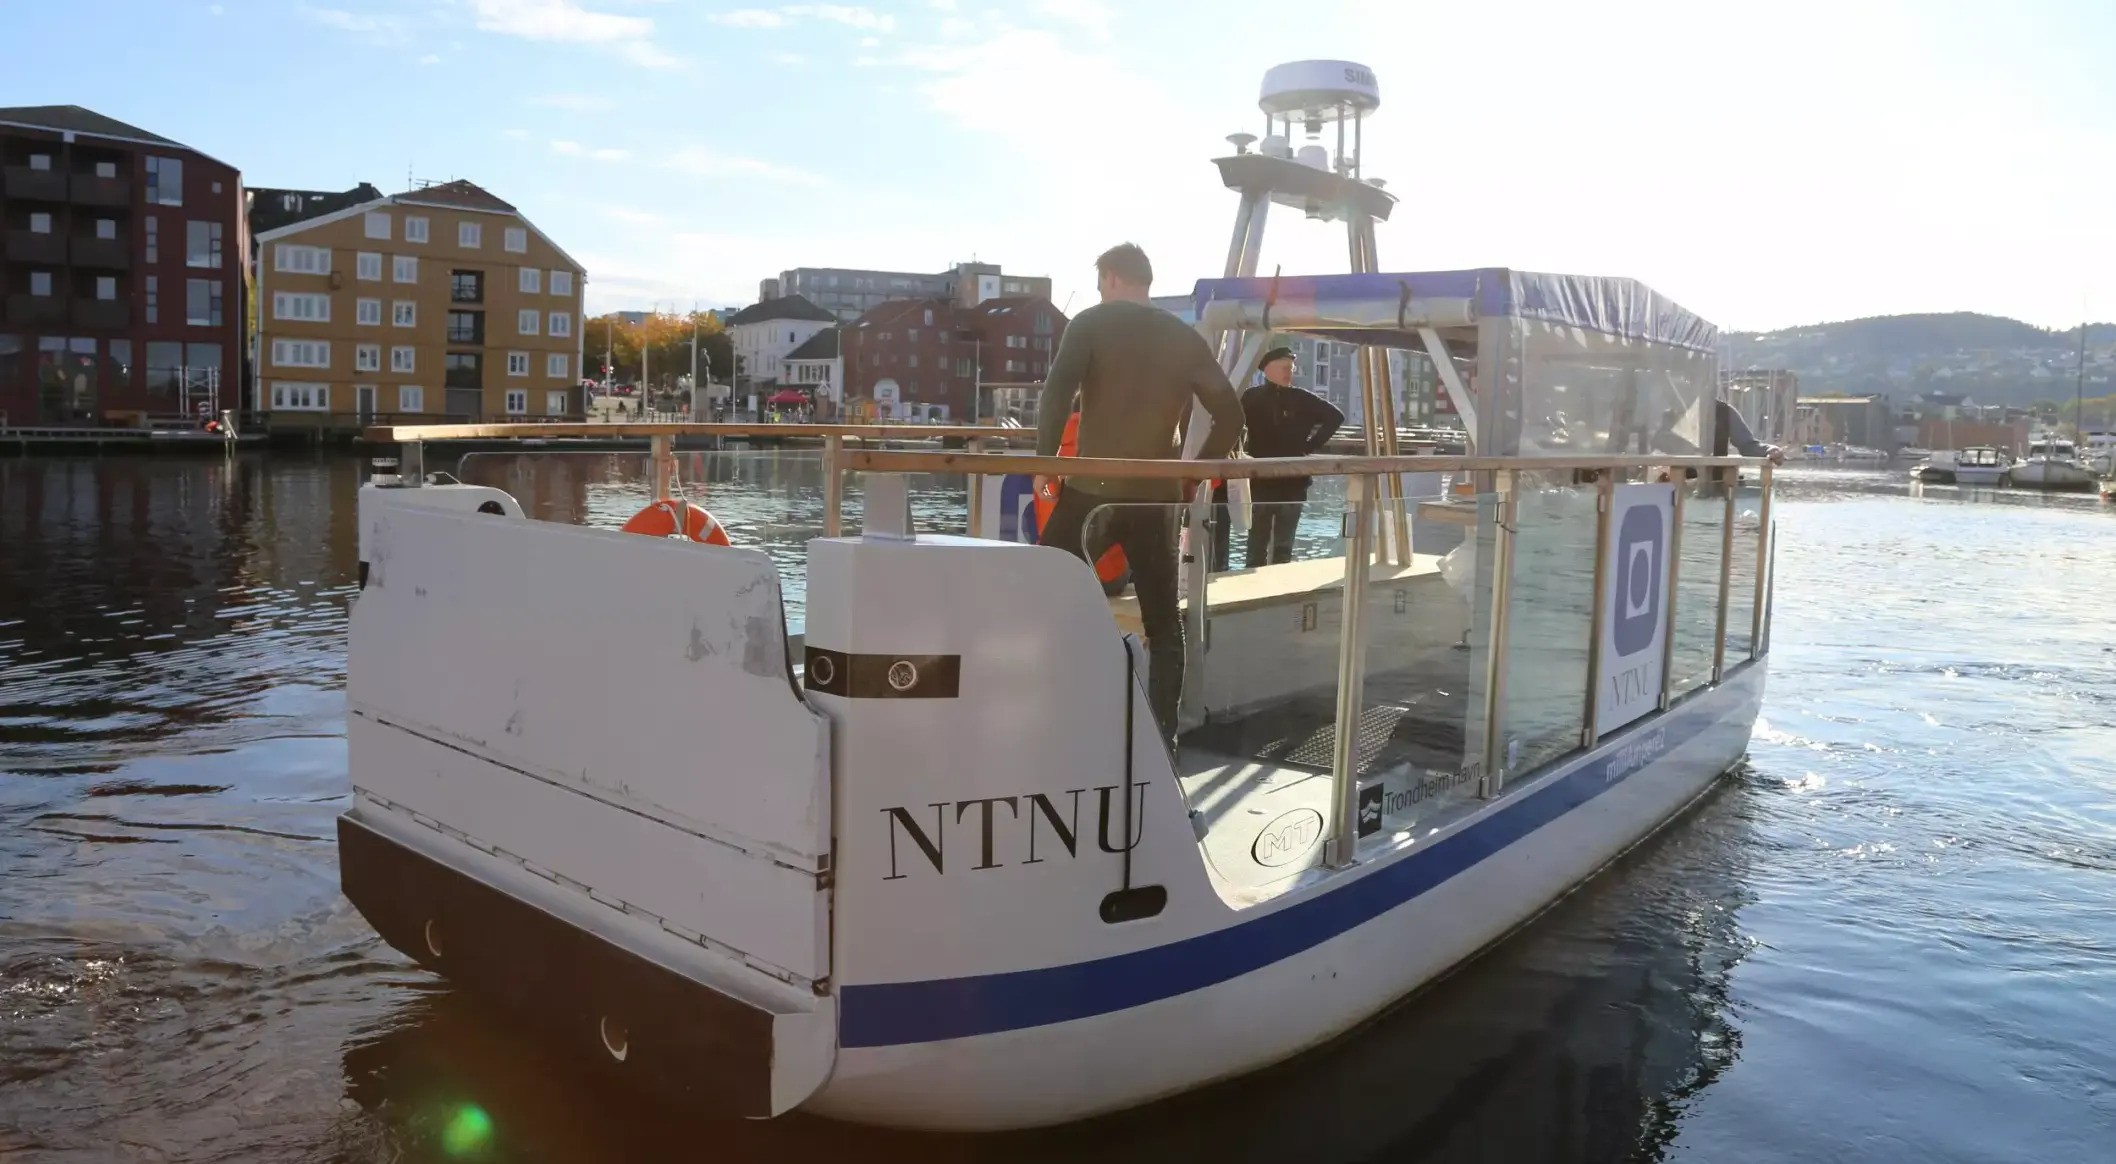
\includegraphics[width=\textwidth]{figures/milliampere.jpg}
    \caption{MilliAmpere 2 driving autonomously in Trondheim harbour \cite{hauglandDetSomHar2022}.}
\end{figure}

\section*{Artificial Intelligence in Autonomous Vehicles}
The word AI gets thrown around a lot these days, so lets clarify what we mean by AI in this context.
As an experienced driver you generally don't have to think a lot when driving a car.
You just have to stay in you lane, keep a safe distance to other vehicles and follow the speed limit.
Most of these things can already be done by a modern car as well, with adaptive cruise control and lane keeping assist.
The ability do this would not be called AI but is rather advanced automation, where a human has defined the rules for what to do.

When something unexpected happens however, you as a driver have to react quickly and make the right decision.
This ability to react to a new and unexpected situations is what is currently missing in autonomous vehicles and is what we refer to as AI when talking about autonomous vehicles.
The problem can be broken into three parts; 1) realizing that something unexpected is happening 2) understanding what that is 3) deciding what to do about it.


\section*{Ferries VS Cars}
Autonomous cars is something that appears to always just be a couple of years away, yet never seems to arrive.
Billions of dollars have been invested into their development but the technology is still not ready for widespread use. 
Why is the development of autonomous ferries any different?

When we start to deploy autonomous vehicles, ehther cars or ferries, there will be a transition period where a human operator is monitoring each vehicle and can take control if needed. 
For autonomous cars, the operator needs to be behind the wheel at all times to be able to react quikly enough and avoid accidents.
Ferries however are a different story.
They move significantly slower than cars, have better overview, cannot cause congestions and do not have to deal with pedestrians in the same way as road vehicles.
An autonomous ferry therefore really only needs to be able to detect that something unexpected is happening, stand still and alert a remote operator and wait for them to take control.
Being a stuck passenger on a ferry waiting for a remote operator to take control might be annoying, but it is not dangerous.
This makes the transition to fully autonomous ferries much more gradual and less risky than for cars.
Being located on the water with line of sight to infrastructure on land also makes it easier to deploy 5G networks that can be used to reliably operate the ferries remotely.

\section*{MilliAmpere 2}
MilliAmpere 2 is a the new research ship from NTNU that is currently being used in the development of autonomous ferries.
With eight cameras, multiple lidars and a radar it is able to observe its surrounding and know how far away other objects are.
Researchers have developed systems that use this data and makes MilliAmpere 2 able to navigate across the harbour autonomously, avoiding other boats.
Currently its behaviour is quite conservative and it is configured to stop when it detects that something unexpected is hapening.
Even though the ferry can be controlled remotely, a human operator is still always present on board to take control if needed.
Citizens of Trondheim have already been able to take rides across the harbour with MilliAmpere 2, and if everything goes according to plan, the ferry will be able to operate fully autonomously in the future.

It is still the early days for autonomous ferries, but the technology is rapidly improving. 
Wheiter or not the optimism around autonomous ferries will play out like the hype around autonomous cars remains to be seen, but for now it appears like the bar is set significantly lower for ferries and that the tech optimists actually might be right.

% \printglossary
% \printbibliography
\title{Reflections}
This text is aimed at the part of the general public that is slightly sceptical towards autonomy, with a goal of explaining why autonomous ferries might be a more realistic technology than autonomous cars.

\section*{Me the Writer}
Acknowledging my own position in relation to the topic is as a good place to start before analyzing the target audience.
As I am taking a PhD in autonomous systems I'm hopefully more knowledgeable about the technology than the average person, and should therefore be aware of the vocabulary and concepts I use to explain the technology.
While researchers might be very pedantic about technical details and technicalities, it is important to note that in order to engage with a broader audience it might be better to avoid the technicalities and focus on the message \cite{kulykPeopleWantReassurance2023}.

As a researcher in the field I'm probably more positive towards autonomous technology than the average person, but knowing how hard it is to implement simingly simple features makes me believe that the technology is still quite far away from being ready for widespread use.

\section*{The Target Audience}
I believe that most people today are familiar with the concept of autonomous vehicles and have some idea of what AI is.
There has for a long time been this idea that autonomous vehicles are just a couple of years away, which I think might have made people a bit sceptical towards the technology, with good reason, as it still has not arrived.
With this in mind I wanted to target that specific underlying scepticism that might be transfered to autonomous ferries as well.
The text does not use a lot of difficult language, and the technical terms used like "lidar" are not necessary to understand in order to get the message of the text.
I do however assume that the reader is familiar with driving a car as I use several comparisons and methaphors that are related to driving, as this can be an effective tool in communicating ideas \cite{gustafssonCognitiveLinguisticsScience2024}.
Young people and paople without a drivers license might therefore not be the best target audience for this text.

\begin{figure}[H]
    \centering
    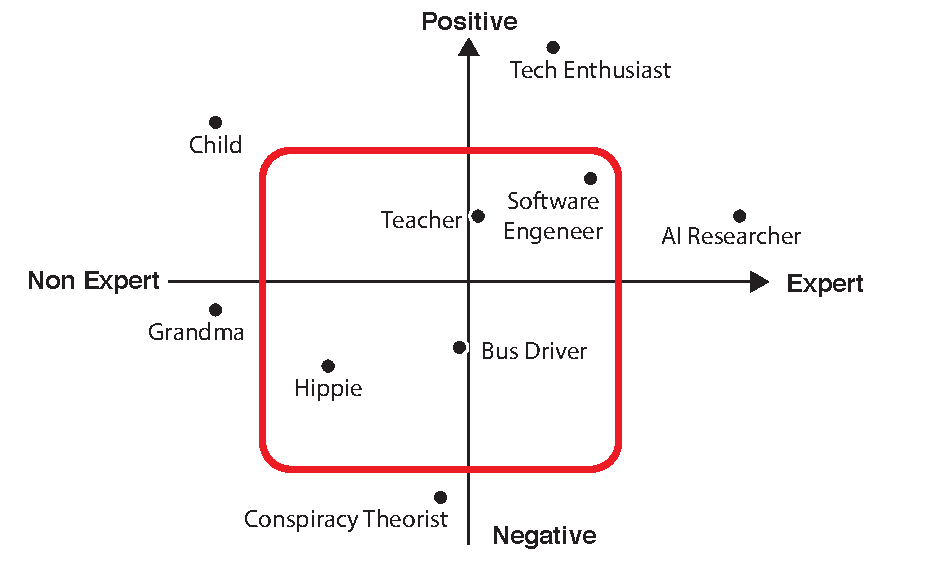
\includegraphics[width=.6\textwidth]{figures/overview.pdf}
    \caption{Visualization of the target audience for this text. The targeg audience is marked in red. The occupations in the figure are mostly based on my own assumptions and are quite stereotypical.}
\end{figure}


This includes avoiding technical jargon and using more narrative driven language to make the text more engaging, as Dahlstrom points out in his article on the topic \cite{dahlstromUsingNarrativesStorytelling2014}.

\section*{How Agency is Framed}
We often use language to describe autonomous systems that imply a level of agency that is not present in the system.
For instance it is fairly common to say that a car "decides" to turn left or that it "understands" that it should stop at a red light.
For people working with autonomous systems these "decisions" are closer to how an elevator "decides" to stop at a floor, in that they are preprogrammed and not the result of any conscious thought, while for the general public the word "decide" might imply a level of agency that is not present in the system.
With the development of more advanced language models, like 


\section*{Political Discussion}











As someone who are working with autonomous systems and are quite positive towards the 






Tech optimists are likely to already be familiar and positive towards the idea of autonomous vehicles and are not 

So called tech optimists are likely to already be familiar and powitive towards the idea of autonomous vehicles, and this text 


\pagebreak
\printbibliography

\end{document}